\chapter{Love, Sex, and Pleasure}

This conversation carries forward the previous inquiry into religion, attention, hurt, and transformation, and turns it toward love. Its precision is not blackboard precision but discriminating precision: love, pleasure, desire, enjoyment, joy, image, hurt, killing, aloneness, and intelligence must not be allowed to blur into one another. The source is J. Krishnamurti's dialogue with Dr. Alan W. Anderson, from material of the Krishnamurti Foundation Trust, curated for this course by LazyingArt LLC with Video2Book.

\section{The Word as a Mirror}

Anderson does not begin with a new subject dropped from outside. He recalls the earlier movement: religion was being considered in relation to attention, hurt, and a transformation not dependent on knowledge or time. Love had appeared at the edge of that conversation. Now he proposes that they explore it.

Krishnamurti immediately slows the word \emph{explore}. Are we exploring intellectually, as though love were an object to be explained, or are we looking into the word so that the word becomes a mirror? This pause is not decorative. It establishes the method of the whole chapter. We do not begin by defining love; we begin by watching what the word reveals in us.

\begin{definition}
In this chapter, a \emph{mirror inquiry} means an inquiry in which the word under examination reveals the movement of the observer: thought, desire, memory, image, fear, hurt, and pursuit.
\end{definition}

The opening movement may be recorded schematically as
\begin{equation}
\text{word ``love''}
\longrightarrow
\text{mirror}
\longrightarrow
\text{observation of oneself}.
\end{equation}
This notation is only a compact guide to the lecture's order. It is not a formal model. The point is that the word is not outside us. If we say ``love,'' the word has to disclose what we actually mean by it.

Krishnamurti then adds the first condition: seriousness. The mind that asks how to acquire love, how to become a successful lover, how to obtain the neighbor's love, is already moving in desire and achievement. Exploration requires a mind that is not trying to turn love into an accomplishment.

\section{The Corruption of the Word Love}

The dialogue next looks at the ordinary range of the word. We say we love God, wife, husband, property, country, books, cinema, and pleasure. One word is made to cover devotion, possession, appetite, entertainment, and national identity. Krishnamurti is not policing vocabulary. He is showing that a corrupted word hides a corrupted inward movement.

This leads naturally to education. Modern education, he says, does not necessarily make the mind serious. It may produce a first-rate specialist and leave the human being shallow. Anderson names the danger: the learned ignoramus. The phrase matters because it marks the separation between information and the understanding of life.

A useful bookkeeping distinction is
\begin{align}
\text{specialization} &\not\Longrightarrow \text{seriousness},\\
\text{knowledge} &\not\Longrightarrow \text{understanding of living}.
\end{align}
The inquiry into love begins only when this split is seen. Otherwise the mind brings its cleverness to the word love and merely makes a more refined confusion.

\section{Is Love Pleasure?}

Krishnamurti now places a series of questions in quick succession. Is love pleasure? Is it the expression of desire? Is it sexual appetite fulfilled? Is it the pursuit of a desired end? Is it identification with family, woman, man, country, or God? Is it something that can be cultivated?

The rhythm is important. He is not trying to produce a definition by negation as a verbal exercise. He is allowing each familiar substitute to show itself. The mind says ``love,'' but the movement may be pursuit, desire, security, identification, or possession.

We can keep this as a cautionary implication:
\begin{equation}
\text{love as pursuit or means}
\longrightarrow
\text{desire or pleasure}
\longrightarrow
\text{division}.
\end{equation}
The arrow does not mean a theorem. It preserves the lecture's warning: when love is made into something to be acquired, used, or fulfilled, it has already entered the field of pleasure and division.

\subsection{Question \& Answer}

\paragraph{Question.}
Can love be cultivated? If I have no love, can I think about it, practice it, work at it, and gradually produce it?

\paragraph{Answer.}
In the lecture's terms, that movement is already a denial of love. A mind that says, ``I lack love, therefore I shall acquire it,'' has made love into an object of becoming. It is moving from lack toward achievement. That is desire, not love.

The same structure appears in religious language. One says one loves God, but if the unknown God is merely the place where worldly pleasures are transferred and purified, the movement is still pleasure. The object has been elevated; the structure has not changed.

\begin{remark}
This is why the chapter must keep ``love of'' under pressure. Love of God, love of country, love of property, and love of success may all carry the same possessive movement unless the mind sees what it is doing.
\end{remark}

\section{Sex, Escape, and the Social Making of Pleasure}

The inquiry now turns from pleasure in general to the identification of love with sex. Krishnamurti is struck by the phrase ``love-making,'' as though the physical act itself were love. He points to cinema, books, pornography, advertisements, stories, and glamour as part of the cultural machinery through which the identification spreads.

Then the question deepens: why has sex become such an enormous affair? The answer is not biological and not moralistic. It is inward and social. If thought is second-hand, if the mind repeats Plato, Aristotle, Buddha, scripture, or any authority without freedom, then intellectually it is unfree. If work is mechanical, if the office bullies, if the factory reduces the human being to repetition, then sex appears as the one region of relief.

The lecture's reasoning can be reconstructed step by step:
\begin{enumerate}
\item The mind is intellectually second-hand when it lives by repetition and authority.
\item Social life becomes mechanical when work, status, and routine dominate living.
\item Emotion then becomes romantic or sentimental, because it seeks relief from mechanical life.
\item Sex appears as the one field in which the person feels some release.
\item What gives relief is then given exaggerated importance.
\end{enumerate}

In compact form:
\begin{align}
\text{second-hand thought} &\longrightarrow \text{intellectual unfreedom},\\
\text{mechanical social life} &\longrightarrow \text{felt imprisonment},\\
\text{romance and sentiment} &\longrightarrow \text{escape},\\
\text{escape through sex} &\longrightarrow \text{sex made enormous}.
\end{align}

\begin{figure}
\centering
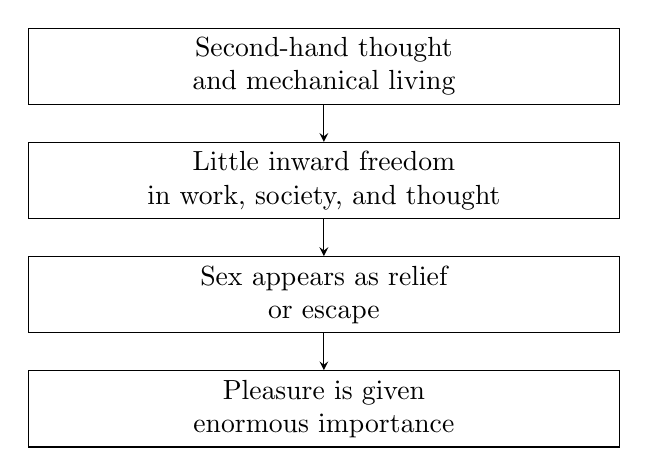
\begin{tikzpicture}[>=stealth]
\node[draw, align=center, text width=0.60\linewidth] (a) at (0,0) {Second-hand thought\\and mechanical living};
\node[draw, align=center, text width=0.60\linewidth] (b) at (0,-1.45) {Little inward freedom\\in work, society, and thought};
\node[draw, align=center, text width=0.60\linewidth] (c) at (0,-2.90) {Sex appears as relief\\or escape};
\node[draw, align=center, text width=0.60\linewidth] (d) at (0,-4.35) {Pleasure is given\\enormous importance};
\draw[->] (a) -- (b);
\draw[->] (b) -- (c);
\draw[->] (c) -- (d);
\end{tikzpicture}
\caption{A transcript-backed reconstruction of the movement by which sex becomes psychologically enormous.}
\end{figure}

At this point religion enters as a contradiction. One part of society advertises and inflates sex; another part condemns, covers, or denies it. Priests may preach celibacy while inwardly burning with desire. Krishnamurti accepts neither indulgence nor repression as understanding. The next question therefore has to be: what is celibacy, and what is chastity?

\section{Celibacy and the Chaste Mind}

The conversation now asks whether celibacy is merely an act, a rule, a vow, an outward abstention, or whether chastity belongs to the mind itself. This is one of the lecture's clearest local obstacles, because religious tradition often treats the outward act as decisive, while Krishnamurti shifts the inquiry inward.

\subsection{Question \& Answer}

\paragraph{Question.}
Is celibacy the outward act, or is chastity a quality of mind?

\paragraph{Answer.}
The lecture rejects the merely outward answer. A mind may take a vow and still be filled with image, fantasy, desire, and conflict. Chastity means a mind that is austere without severity, innocent because it is not hurt, and free from the image of the woman, the man, the act, and its own appetite.

\begin{table}
\centering
\begin{tabular}{|p{0.42\linewidth}|p{0.42\linewidth}|}
\hline
\textbf{Outward celibacy} & \textbf{Chaste mind} \\
\hline
May be a vow, rule, or religious discipline. & Is a quality of mind, not merely an act. \\
\hline
May coexist with burning desire and image. & Has no inward image of possession, sex, or appetite. \\
\hline
Can become severe, proud, or repressive. & Is austere without brutality or severity. \\
\hline
Does not by itself end conflict. & Is innocent because it is not hurt. \\
\hline
\end{tabular}
\caption{The lecture's distinction between outward celibacy and inward chastity.}
\end{table}

This returns the chapter to the earlier inquiry into hurt. A chaste mind would not be hurt because it is not organized around an image. It has no picture of itself, another, or its own appetite. Anderson connects this to the old idea that the fall begins with imagination. Krishnamurti does not turn that reference into doctrine. He keeps the point exact: where image operates, conflict operates.

We can summarize the inward criterion as
\begin{equation}
\text{chastity}
\longleftrightarrow
\text{no hurt, no image, no imaginative possession}.
\end{equation}
The double arrow is a note-making convenience, not a definition imposed from outside. It keeps together the qualities named in the dialogue.

\section{Pleasure, Enjoyment, and Joy}

Now Krishnamurti comes back to the central discrimination. Love cannot be understood unless pleasure is understood. Pleasure divides. Enjoyment does not divide when it ends in the moment. Joy does not divide, and it cannot be invited or held.

The temporal movement is decisive. There is enjoyment: a meal, a sunset, a tree, a face. If it ends there, it is simply enjoyment. But thought remembers, carries it over, and asks for repetition. At that point enjoyment has become pleasure.

\begin{equation}
\text{enjoyment}
+
\text{thought carrying it over}
+
\text{demand for repetition}
\longrightarrow
\text{pleasure}.
\end{equation}

From there the next movement follows:
\begin{equation}
\text{pleasure}
\longrightarrow
\text{division}.
\end{equation}

\subsection{A Worked Example: How Enjoyment Becomes Pleasure}

Consider the ordinary example of seeing a beautiful sunset.

\begin{enumerate}
\item There is immediate perception.
\item In that moment there is enjoyment.
\item Thought remembers the enjoyment.
\item Thought says, in effect, ``I want that again.''
\item The remembered enjoyment becomes pursuit.
\item Pursuit is pleasure.
\item Because the pursuit is now organized around ``me'' and ``mine,'' it divides.
\end{enumerate}

The worked example is simple, but it carries the lecture's mathematical spine: the transformation occurs through time, memory, and repetition. Enjoyment is not condemned. The danger lies in continuation by thought.

\begin{figure}
\centering
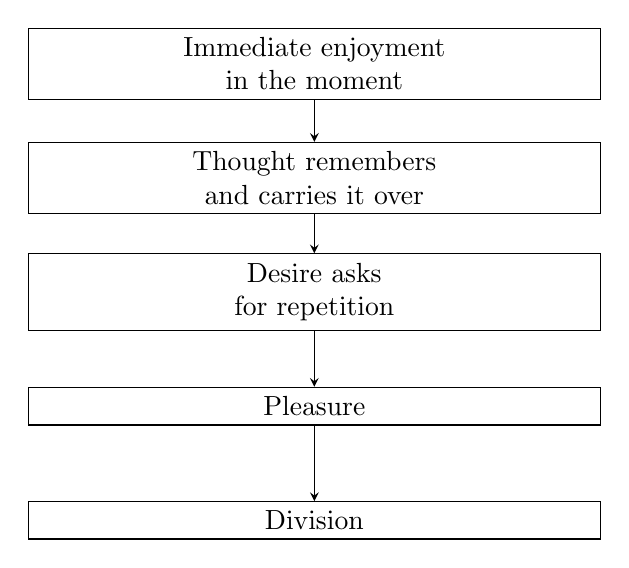
\begin{tikzpicture}[>=stealth]
\node[draw, align=center, text width=0.58\linewidth] (a) at (0,0) {Immediate enjoyment\\in the moment};
\node[draw, align=center, text width=0.58\linewidth] (b) at (0,-1.45) {Thought remembers\\and carries it over};
\node[draw, align=center, text width=0.58\linewidth] (c) at (0,-2.90) {Desire asks\\for repetition};
\node[draw, align=center, text width=0.58\linewidth] (d) at (0,-4.35) {Pleasure};
\node[draw, align=center, text width=0.58\linewidth] (e) at (0,-5.80) {Division};
\draw[->] (a) -- (b);
\draw[->] (b) -- (c);
\draw[->] (c) -- (d);
\draw[->] (d) -- (e);
\end{tikzpicture}
\caption{Enjoyment becomes pleasure when thought carries it over and seeks repetition.}
\end{figure}

Joy is treated even more delicately. Krishnamurti says that the moment joy is recognized as joy, it is gone. Anderson brings in a remembered line from Blake to point toward joy that is not held. The chapter should not become literary commentary here. The important point is that joy is falsified when thought tries to invite, possess, or repeat it.

\begin{table}
\centering
\begin{tabular}{|p{0.27\linewidth}|p{0.27\linewidth}|p{0.27\linewidth}|}
\hline
\textbf{Joy} & \textbf{Enjoyment} & \textbf{Pleasure} \\
\hline
Cannot be invited; recognition already alters it. & Immediate, complete when it ends in the moment. & Continuity of enjoyment through thought and repetition. \\
\hline
Not divisive. & Not divisive when it is not carried over. & Divisive because it becomes pursuit and possession. \\
\hline
Not produced by method. & Belongs to direct contact with what is. & Belongs to memory, desire, and becoming. \\
\hline
\end{tabular}
\caption{A compact reconstruction of the lecture's distinction between joy, enjoyment, and pleasure.}
\end{table}

This distinction also explains why the lecture now turns to nationalism, ambition, and killing. Pleasure divides; division does not remain private.

\section{Love and Killing Cannot Be Joined}

Krishnamurti next asks us to look at the forms division takes: pride, nationalism, power, ambition, religious position, and killing. A person may speak of love of country, but that love may be ready to kill. A priest may speak of God and yet be ambitious. A civilization may speak of morality while perfecting war.

The point is not an abstract pacifist slogan. It is a test of the word love. If the mind is ambitious, if it wants power, if it participates in organized killing, what does it mean when it says love?

\begin{proposition}
Within this lecture, love cannot be joined to designed killing, ambition, and organized division.
\end{proposition}

\begin{proof}
The reasoning proceeds through contradiction. Pleasure is divisive. Division appears as pride, nationalism, possession, ambition, and power. These movements sustain violence and organized killing. A mind that participates inwardly in that division may still use the word love, but the word has lost its substance. Therefore the inquiry into love must also inquire into killing.
\end{proof}

The anecdote of the Buddhist couple in Ceylon tests this contradiction in ordinary life. They say they do not kill, yet they eat meat and shift responsibility by changing butchers. The point is not sectarian criticism. It is the human capacity to separate action from responsibility. The same separation appears in the larger world: armies prepare to kill, governments design enemies, the earth is polluted, species are destroyed, and yet people continue to use the language of love.

\subsection{Question \& Answer}

\paragraph{Question.}
If one is serious and one loves, does that mean one will never act when violence occurs?

\paragraph{Answer.}
The lecture does not give a fixed answer in advance. Krishnamurti distinguishes designed killing from intelligent action in the moment. If someone is attacked, intelligence born of compassion acts then. But to prepare systems of killing, organize enemies, and build violence as policy is not intelligence. It is design, fear, and division.

The contrast is
\begin{align}
\text{compassion} &\longrightarrow \text{intelligence} \longrightarrow \text{action in the situation},\\
\text{fear and division} &\longrightarrow \text{designed killing} \longrightarrow \text{organized violence}.
\end{align}

This is why Anderson's phrase ``killing by design'' is so important. The lecture is not asking for a theoretical answer to every possible emergency. It is exposing the inward and institutional preparation to kill.

\section{Education, Seeing, and Aloneness}

Anderson now brings the inquiry to education. A student comes and asks, ``What must I do?'' Krishnamurti sees the trap. The question often asks for a means. If I can be given a method, I can add the method to my present structure and continue as before. But this inquiry has been undermining that whole structure. Seeing is not the first step of a method; seeing danger is action.

\begin{align}
\text{seeing danger} &\longrightarrow \text{immediate action},\\
\text{not seeing danger} &\longrightarrow \text{continuity of thought}.
\end{align}

Here we should hear the connection with pleasure. If I see the danger of thought continuing pleasure, I act. If I do not see it, I carry on. No method can substitute for that seeing.

\subsection{Question \& Answer}

\paragraph{Question.}
What am I to do in this world?

\paragraph{Answer.}
Krishnamurti first reframes the question: what is my place in this world? The answer begins with the fact that the world is not merely outside. The world of corruption, war, superstition, killing, and lack of love is also the movement of the self. If I am that movement, my relationship to the world is participation in it. If that movement ends, relationship has another quality.

The next word is \emph{alone}, but it must be protected from misunderstanding. Aloneness is not isolation, withdrawal, or an inward tower. Isolation is produced by ambition, nationalism, family possession, fulfillment, and self-centered activity. Aloneness comes when those movements are seen as false and are negated without violence.

\begin{figure}
\centering
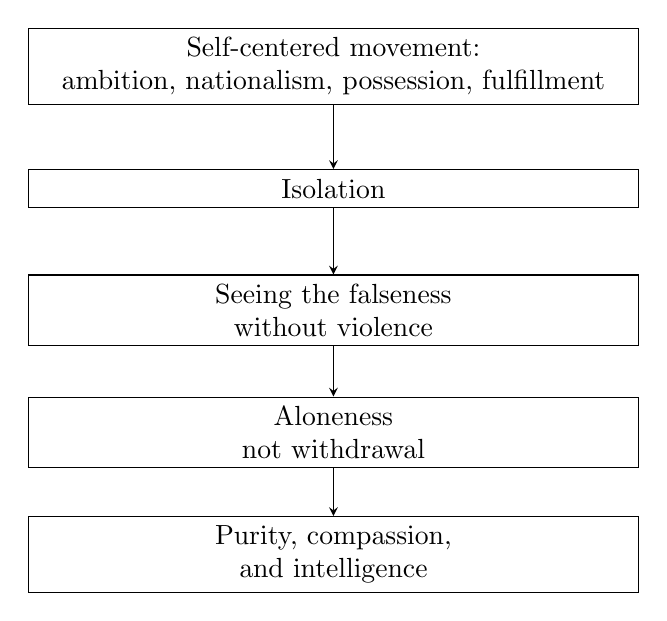
\begin{tikzpicture}[>=stealth]
\node[draw, align=center, text width=0.62\linewidth] (a) at (0,0) {Self-centered movement:\\ambition, nationalism, possession, fulfillment};
\node[draw, align=center, text width=0.62\linewidth] (b) at (0,-1.55) {Isolation};
\node[draw, align=center, text width=0.62\linewidth] (c) at (0,-3.10) {Seeing the falseness\\without violence};
\node[draw, align=center, text width=0.62\linewidth] (d) at (0,-4.65) {Aloneness\\not withdrawal};
\node[draw, align=center, text width=0.62\linewidth] (e) at (0,-6.20) {Purity, compassion,\\and intelligence};
\draw[->] (a) -- (b);
\draw[->] (b) -- (c);
\draw[->] (c) -- (d);
\draw[->] (d) -- (e);
\end{tikzpicture}
\caption{Isolation is produced by self-centered movement; aloneness appears when that movement is seen and negated.}
\end{figure}

Krishnamurti says that such aloneness is pure. It is not my purity or your purity. Anderson adds the image of fullness from Sanskrit, but the main point remains simple: aloneness is the quality of a mind that has not withdrawn from the world and yet is no longer inwardly made of its corruption.

The final practical test concerns money entrusted to a friend who later denies receiving it. What is love there? It is not sentimental forgiveness that merely walks away. Love is intelligence, and intelligence is sensitivity to the situation. If recovery is possible, intelligence may act. If one acts from hurt, resentment, or a fixed conclusion, the action is insensitive.

The final chain is therefore best written as
\begin{equation}
\text{love or compassion}
\longrightarrow
\text{intelligence}
\longrightarrow
\text{sensitivity to the situation}
\longrightarrow
\text{appropriate action}.
\end{equation}
The last term must remain open. The lecture refuses a precomputed answer. The situation, met with sensitivity, discloses what action is.

The conversation then points forward. Anderson raises conscience and consciousness; Krishnamurti agrees that this must be investigated next. The chapter therefore closes not with a system, but with the next question already visible.

\section{Summary}

The movement of the chapter is one inquiry with several tests. First, the word love is made into a mirror. Then the corrupted uses of the word are exposed: God, country, property, sex, success, and pleasure. The question ``Is love pleasure?'' opens the main investigation, and the answer cannot be verbal. The mind must see how desire, cultivation, pursuit, and identification imitate love.

Sex becomes enormous because much of life is inwardly unfree. Outward celibacy does not solve the problem; chastity is a quality of mind without hurt, image, or imaginative possession. The chapter's central distinction is that enjoyment becomes pleasure when thought carries it over and demands repetition. Pleasure divides.

That division expands into nationalism, ambition, power, and killing. Therefore love cannot be examined apart from violence. A serious mind cannot make killing into a design and still speak coherently of love. Yet the lecture does not offer formulas for action. Compassion gives rise to intelligence, and intelligence is sensitive to the actual situation.

Finally, education is brought back into the question. The demand ``What must I do?'' often hides a search for method. Krishnamurti's answer is sharper: seeing danger is action. When the movements of ambition, possession, nationalism, and self-fulfillment are seen and negated, the mind is alone, not isolated. In that aloneness the lecture locates purity, compassion, intelligence, and the possibility of love.